\documentclass{article}
\renewcommand{\rmdefault}{psbx}
\usepackage[utf8]{inputenc}
\usepackage[T1]{fontenc}
\usepackage{textcomp}
\usepackage{eulervm}
\usepackage{amsmath}
\usepackage{amssymb}

\setlength{\textwidth}{160mm}
\setlength{\oddsidemargin}{0mm}
\setlength{\parindent}{0 mm}

\newcommand{\bfa}{{\bf a}}
\newcommand{\bfb}{{\bf b}}
\newcommand{\bfm}{{\bf m}}
\newcommand{\bfs}{{\bf s}}
\newcommand{\bfz}{{\bf z}}
\newcommand{\E}{{\mathbb E}}
\newcommand{\V}{{\mathbb V}}

\usepackage{tikz}
\usetikzlibrary{arrows,shapes,backgrounds,patterns,fadings,decorations.pathreplacing,decorations.pathmorphing}
\tikzset{>=stealth'}

\title{The Pendulum Task}
\author{Jonas Umlauft}
\date{July 10th 2014}

\begin{document}

\maketitle
\begin{center}
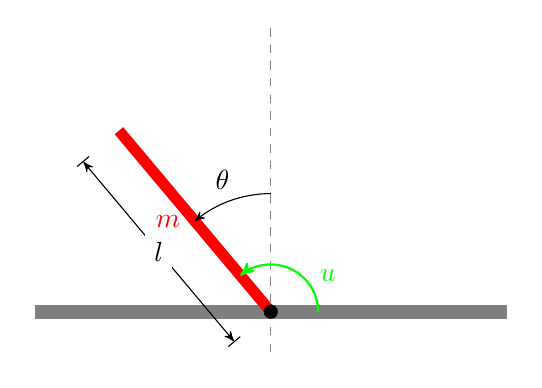
\begin{tikzpicture}[scale=3]
\def\l {1}
\def\ang {130}
    \draw[gray,line width = 5] (-1,0)--(1,0);
    \draw[gray, dashed] (0,1.2*\l)--(0,-0.2*\l);
    % Pendulum
    \draw[red,line width = 4] (0,0) -- (\ang:\l) node[midway,anchor = east] {$m$};
    \fill[black] (0,0) circle(0.03cm);
    \draw [->] ([shift=(90:0.5*\l)]0,0)  arc (90:\ang:0.5*\l) node[right = 10, above = 8] {$\theta$};
	\draw [->,green,thick] ([shift=(0:0.2*\l)]0,0)  arc (0:\ang:0.2*\l) node[right = 25] {$u$};
	\draw[|<->|,draw=black] ([shift=(\ang+90:0.2*\l)]0,0) -- ([shift=(\ang+90:0.2*\l)]\ang:\l) node[fill=white, midway]  {$l$};

\end{tikzpicture}  
\end{center}
\subsection*{General}
The pendulum system consists of pendulum (uniformly distributed mass $m$, length $l$) which is attached frictionless on one end. The pendulum angle, $\theta$, is measured anti-clockwise
from upright. A external moment $u$ acting on the pendulum at the origin can be applied. Typical values are: $m=1{\rm kg}$,  $l=1{\rm m}$.
Two task can be considered
\begin{itemize}
\item For the pendulum starting in the upright position $ \theta =0$, the task is to \textbf{stabilize} it in this position. 
		This can be achieved using a linear controller or a nonlinear controller.
\item For the pendulum starting  in the hanging down position $ \theta =\pi$, the task is to \textbf{swing-up} in the upright position and stabilise there. 
	 This can only be achieved using a nonlinear controller.
\end{itemize}


\subsection*{Dynamics}
The following equilibrium of moments acting on the pendulum must be fulfilled at all times:
\begin{align*}
\frac{d^2 \theta}{dt^2}I = \frac{1}{2} mgl\sin (\theta) +u
\end{align*}
where $I = \tfrac{1}{3} ml^2$ is the moment of inertia.

The state vector is defined as $\bfz = \begin{bmatrix} \dot{\theta} & \theta \end{bmatrix}^T$, thus the differential equation is given as following
\begin{align*}
\frac{d\bfz}{dt}= \left\{ \begin{array}{l}
\frac{3}{ml^2} \left(\frac{mgl}{2} \sin (z_2) +  u \right) \\
 z_1
\end{array}\right. ,
\end{align*}


\subsection*{Linearized Dynamics}

Linearising the dynamics around the goal state $\bfz =\begin{bmatrix} 0 & 0 \end{bmatrix}^T$ , we can write the
following approximation
\[
\frac{d\bfz}{dt}\;\simeq\;(A\bfz+B u),\qquad
A\;=\;\begin{bmatrix}

0&\frac{3g}{2l}\\
1&0 \end{bmatrix},\qquad
B\;=\; \begin{bmatrix} \frac{3}{ml^2} \\ 0\end{bmatrix}
\]


\subsection*{Loss Function}
Currently exist two implementations for the loss functions
\begin{itemize}
\item The instantaneous loss is given by
\[
F\;=\;1-\exp(-\frac{d^2}{2a^2}),
\]
were  $a$ is the \emph{width} parameter of the cost function and $d$ is  the Cartesian distance between the tip of the pendulum and the point at distance $\ell$ above the origin,
	   The squared distance is
	\[
	d^2\;=\;(\ell\sin\theta)^2+(\ell-\ell\cos\theta)^2
	\;=\;(\tilde\bfz-\mu)^\top Q(\tilde\bfz-\mu),
	\]
	where $\tilde\bfz$ is $\bfz$ augmented by two coordinates $\sin\theta$ and $\cos\theta$  with 
		\[
	Q\;=\;\begin{bmatrix}0&0&0&0 \\ 0&0&0&0 \\ 0&0&l^2&0 \\ 0&0&0&l^2 \end{bmatrix},\qquad
	\mu\;=\;\begin{bmatrix} 0 \\ 0 \\ 0 \\ 1 \end{bmatrix}.
	\]
	Note that the instantaneous loss does not depend on the speed variable $\dot\theta$.
	This is currently implemented in \textit{loss.m}	
	\item The instantaneous loss is given by
	\begin{align*}
	F\;=\; (\cos (\theta) +1)/2
	\end{align*}		
	i.e. the angular distance to the upright position. This is currently implemented in \textit{loss2.m}.
\end{itemize}
The \emph{expected loss}, averaging over the possibly uncertain states
is therefore
\[
\E[F(\tilde\bfz)]\;=\;1-\int F(\tilde\bfz)p(\tilde\bfz)d\tilde\bfz,
\]
which can be evaluated in closed form for Gaussian $p(\tilde\bfz)$, see
reward.pdf. Since the augmented state $\tilde\bfz$ will not generally
be Gaussian even if $\bfz$ is Gaussian, we project on to the closest
Gaussian by matching first and second moments.
\end{document}

